\section{Abstract Syntax Tree en Go}
\textit{Go} provee una serie de paquetes que permiten trabajar con código fuente escrito en ese lenguaje de programación, facilitando la creación de \textbf{árboles de sintáxis abstracta}, para el análisis o manipulación de los mismos.
Al ser provisto oficialmente por los creadores, no es necesario definir la gramática para alguna otra herramienta como ANTLR o VEEEER.
Además, esto nos asegura que se soportan todas las estructuras que componen el lenguaje y se encuentran definidas en la especificación del mismo.

\begin{figure}[H]
  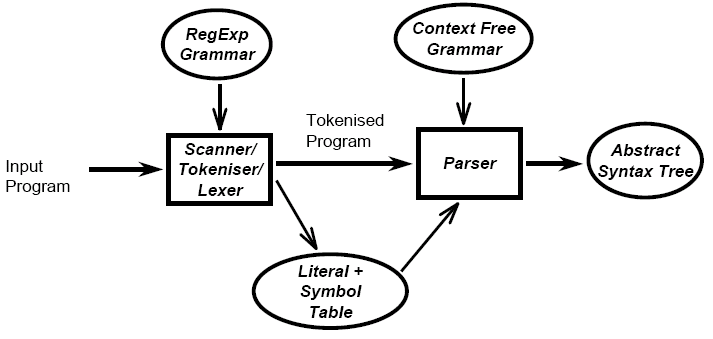
\includegraphics[width=12cm]{implementation/parsingpipeline}
  \centering
  \caption{Creación de un AST desde código fuente}
\end{figure}

En la figura X se establece la correlación entre las etapas del proceso de creación de un AST a partir de código fuente y los paquetes provistos en el lenguaje de programación.
La función de cada uno de estos, y su participación en el proceso, se indica a continuación:
\begin{itemize}
  \item \textbf{go/token} Contiene
  
  \item \textbf{go/scanner}
  
  \item \textbf{go/ast}
  
  \item \textbf{go/parser}
\end{itemize}
